%%%%%%%%%%%%%%%%%%%% book_ch08.tex (CN book shell; 第8章正文) %%%%%%%%%%%%%%%%%%%%
% 与英文 Springer SNmono 样本同构：全书书名为 proposal 总标题；
% 第1--7、9章仅列章节名；第8章为已起草正文。中文用 ctexbook 承载中文字体。
\documentclass[UTF8,a4paper,openany]{ctexbook}

\usepackage{graphicx}
\usepackage{booktabs}
\usepackage{multirow}
\usepackage{tabularx}
\usepackage{enumitem}
\usepackage{amsmath,amssymb}
\usepackage{algorithm}
\usepackage{algpseudocode}
\usepackage{xcolor}
\usepackage[numbers,sort&compress]{natbib}
\usepackage{hyperref}
\usepackage{geometry}
\geometry{margin=2.5cm}

\graphicspath{{figures/}{figures/ch08/}}

\newcommand{\StubChapter}[1]{%
  \chapter{#1}%
  \vspace{1.5em}%
  \noindent\textit{本章正文将在全书定稿中提供。}%
  \clearpage
}

\begin{document}

% 全书书名页（对齐 SNmono：书名 + Springer Nature；不写个人作者）
\thispagestyle{empty}
\vspace*{2em}
{\Huge AI驱动的无人机建筑巡检\par}
\vfill
{\Large Springer Nature\par}
\clearpage

\tableofcontents

% ----- 第1--7章：仅列 proposal 章节名 -----
\StubChapter{无人机建筑巡检导论}
\StubChapter{面向数据采集的无人机任务规划}
\StubChapter{复杂环境下的无人机运动规划}
\StubChapter{建筑三维重建}
\StubChapter{数据集构建与基准}
\StubChapter{面向建筑巡检的人工智能模型}
\StubChapter{面向建筑监测的GIS集成}

% ----- 第8章：已起草正文 -----
%%%%%%%%%%%%%%%%%%%%% ch08_cn.tex — 专著综合稿（非单篇论文复述） %%%
\chapter{巡检分析中的数字孪生与大语言模型}
\label{ch:llm-dt}

\noindent\textit{摘要：}本章展开无人机巡检流水线的决策层：在规划、重建、检测与 GIS 锚定之后，大语言模型与视觉—语言模型如何支撑孪生上的诊断与运维决策？叙事遵循专著常见的\textbf{先广后专}：先综述 LLM/VLM 在建筑巡检与设施管理中的广泛用法，再阐明专业巡检相对通用聊天的约束，最后落到孪生接地的「观测记录 / 资产护照 / 拓扑检索 / 智能体 / 报告交付」框架。叙述综合社区工作与课题组贡献；资产中心 RAG 仅作众多路径中的一个工作示例。

\vspace{0.8em}

%%%%%%%%%%%%%%%%%%%%%%%%%%%%%%%%%%%%%%%%%%%%%%%%%%%%%%%%%%%%%%%%%%%%%%
\section{面向建筑巡检的数字孪生}
\label{sec:ch8-dt}

\subsection{本章在全书中的位置}
专著按一条流水线展开：第2--3章负责任务与运动规划，第4章重建几何，第5--6章数据集与缺陷感知，第7章 GIS/GeoBIM 为资产赋予城市尺度地址。这些章节单独都还不能回答：「哪些板块处于跨层渗水路径？」「如何起草一份工程师可审计的维修简报？」——这属于\textbf{决策层}：把孪生实体接到语言、检索，以及越来越多的工具型智能体。

\begin{figure}[t]
\centering

\includegraphics[width=0.9\textwidth]{framework_overview_overall.pdf}
\caption{巡检智能的书级视图。本章聚焦消费前几章孪生与感知产物的语言、检索与决策层。}
\label{fig:ch8-framework}
\end{figure}

\subsection{开场场景：纯几何孪生答不了的问题}
设想物流仓完成季度无人机巡检后，设施经理提出三个看似平常、方法上却很苛刻的问题：
\begin{enumerate}[leftmargin=*]
\item \emph{空间类.}「把东立面严重度中等以上的空鼓 Asset-ID 全部列出来。」
\item \emph{多跳/传播类.}「若 A-07 板块上方两层出现潮湿，下一步应检查哪些邻域资产？」
\item \emph{聚合/规划类.}「起草一份吊篮排程，优先处理同时有 RGB 裂缝与 IR 异常的资产，并给出我能在孪生中打开的证据。」
\end{enumerate}
网格浏览器可以上色，检测器可以画框，但二者都不会产出\textbf{可审计}的自然语言答案——把症状、Asset-ID、邻域与维修优先级绑定起来。本章其余部分就是在建设这层缺失能力。

\subsection{语言可用的孪生必须提供什么}
几何孪生回答「在哪里」。决策就绪孪生还必须提供：（1）稳定资产标识；（2）每条观测的出处（传感器、时间、检测器）；（3）支持传播阅读的邻接关系。缺了这些，语言模型只能对着散乱文件闲聊——流畅，但对设施管理（FM）不可审计。

建设领域数字孪生综述强调：孪生不是单纯的三维浏览器，而是连接建成几何、语义与运维的演化信息系统~\cite{boje2020,opoku2021,lu2020}。UAV--BIM 巡检综述很早提出自动化议程~\cite{zhang2022}。本课题组中，张纪涵等展示了耦合无人机感知与 GeoBIM 的高精度缺陷管理数字孪生~\cite{zhang2025}；Det-Recon-Reg 将检测、重建与配准封装为大规模巡检框架~\cite{yang2025detreconreg}。孪生应用也不限于立面，例如大型工地工人监测~\cite{han2025}。BIM 内多智能体虚拟建模进一步表明：孪生正成为主动信息系统，而不只是静态视图~\cite{lee2025multiagentvbm}。这些工作为下文语言层提供几何与标识前提。

\begin{figure}[t]
\centering
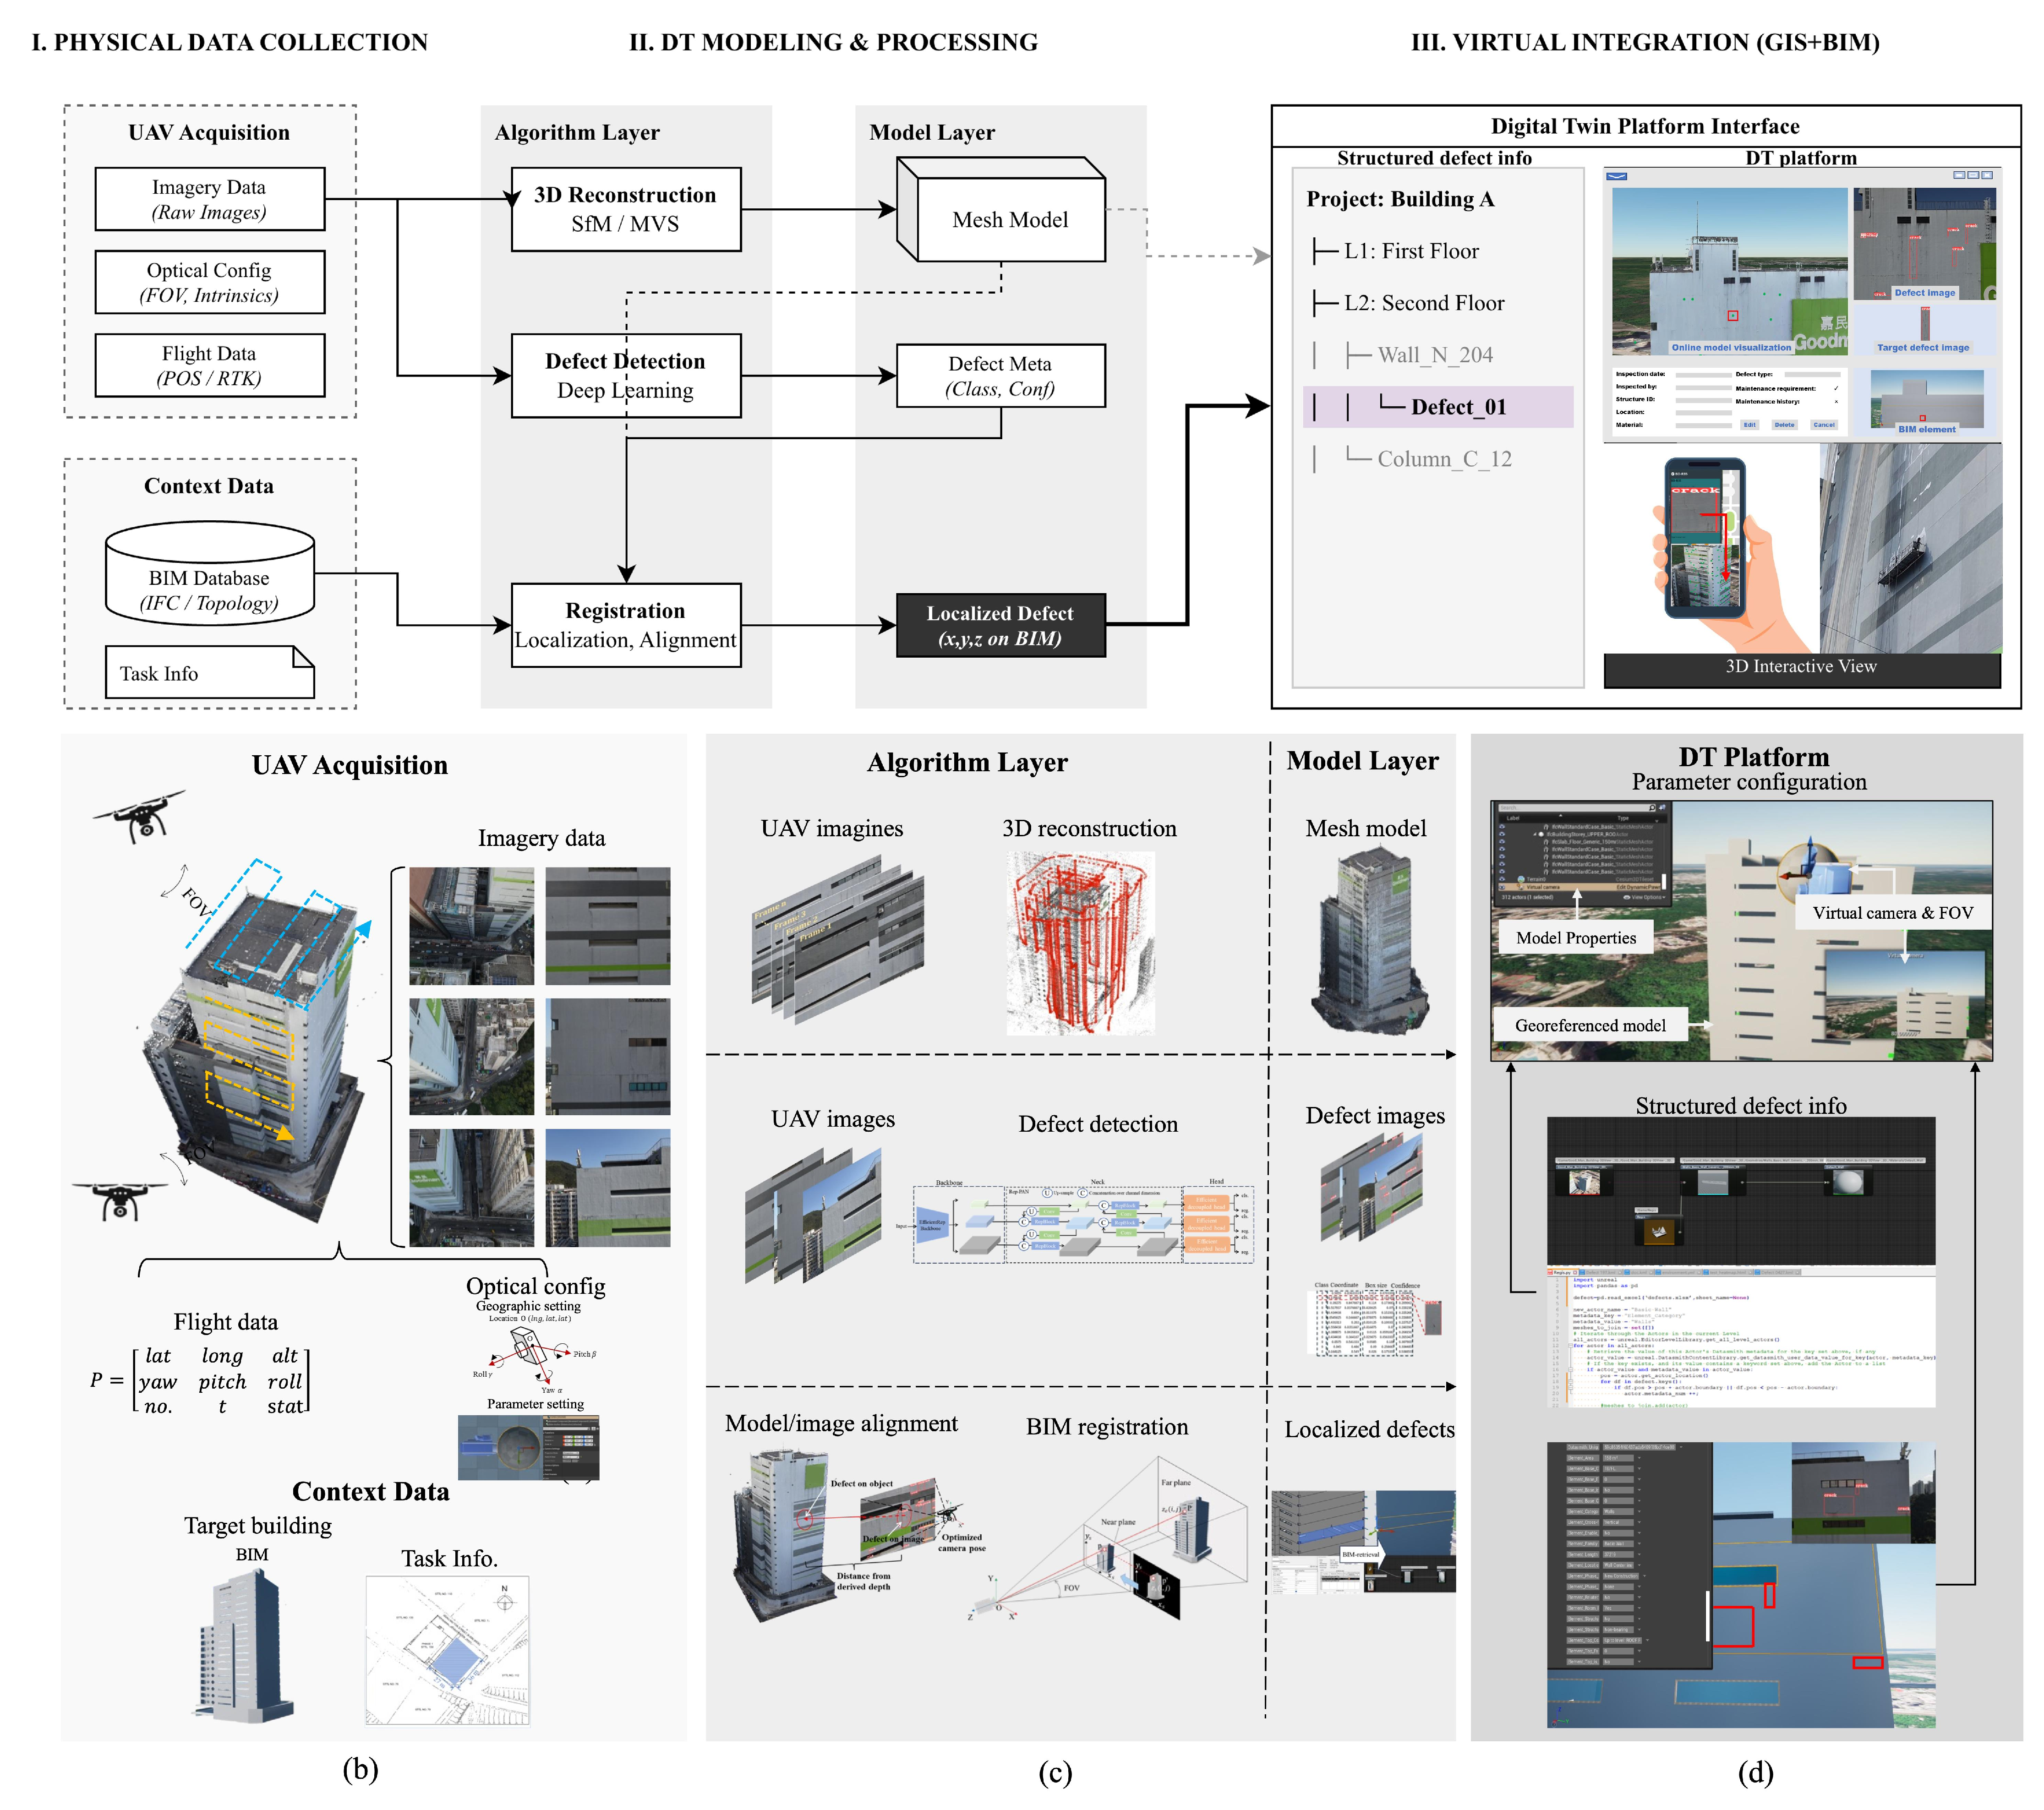
\includegraphics[width=0.88\textwidth]{dt_modeling_pipeline.pdf}
\caption{前几章深入展开的无人机→孪生建模路径。此处将其视为语言分析的\textbf{输入接口}。}
\label{fig:ch8-dt-pipeline}
\end{figure}

\subsection{仅靠语言填不平的缺口}
现场项目中常见三类缺口：
\begin{itemize}[leftmargin=*]
\item \textbf{可视化 $\neq$ 推理.} 看见裂缝并不等于解释跨层风险。
\item \textbf{缺少 provenance.} 没有传感器/时间/检测器戳记，生成建议无法审计。
\item \textbf{缺少有纪律的自然语言接口.} 对着 PDF 闲聊会虚构 Asset-ID；对着孪生闲聊却无引用规则，只会更自信地犯同样错误。
\end{itemize}
因此第8章承诺：结构化知识单元、接地的 LLM/VLM 生成、约束报告与决策指标——而不是把聊天机器人贴到点云上。

\paragraph{过渡.}
因此我们先从\textbf{广泛}层面梳理大模型已在巡检与设施实践中如何使用，再收束到孪生接地立面诊断的\textbf{专业}要求。

%%%%%%%%%%%%%%%%%%%%%%%%%%%%%%%%%%%%%%%%%%%%%%%%%%%%%%%%%%%%%%%%%%%%%%
\section{面向土木工程应用的大语言模型基础}
\label{sec:ch8-llm-foundations}

\subsection{广角：大模型已在巡检中帮忙的地方}
大语言模型（LLM）与视觉—语言模型（VLM）进入建筑巡检，并不是单一产品，而是人、文档、模型与机器之间的一类接口族~\cite{saka2024gptconstruction,ma2026tenquestions}。最宽的层面上，实践者主要用它们完成五类重复性工作：

\begin{enumerate}[leftmargin=*]
\item \textbf{文档与规范问答.} 人员询问规范版本、安全手册与运维手册；检索增强生成（RAG）通常优于仅依赖参数记忆~\cite{joffe2025buildingcodes,lee2024ragsafety,krutli2025fmrags}。
\item \textbf{BIM 与模型导航.} 自然语言助手在设计/建成 BIM 中定位对象、属性与关系~\cite{zheng2023bimassistant,guo2025bimllmquery}。
\item \textbf{缺陷对话与分诊.} 混合 RAG 支持围绕缺陷记录与管理日志的对话~\cite{jeon2025hybridrag}，起草供人工审阅的优先级候选。
\item \textbf{报告起草与摘要.} 模型把巡检笔记、照片说明与检查表结果整理为工程师再编辑的初稿。
\item \textbf{面向孪生与机器人的任务经纪.} 新兴智能体把用户意图译为工具调用：读取孪生、请求机器人补拍，或在批准后暂存更新~\cite{luo2025llmdtrobot,gao2026ifcagent,rawat2025llmmas,lee2025multiagentvbm}。
\end{enumerate}

\begin{table}[t]
\centering
\caption{建筑巡检与设施管理中 LLM/VLM 的广义应用模式（专业化之前的版图）。}
\label{tab:ch8-llm-modes}
\begin{tabular}{p{2.6cm}p{3.6cm}p{5.4cm}}
\toprule
模式 & 典型输入 & 典型输出 \\
\midrule
规范/手册问答 & 法规文本、手册 & 带引用条款、检查清单 \\
BIM 导航 & IFC/BIM 对象、查询 & 对象关联答案 \\
缺陷对话 & 日志、影像、历史工单 & 分诊笔记、假设 \\
报告起草 & 笔记 + 照片说明 & 可编辑报告草稿 \\
孪生/机器人智能体 & 孪生状态 + 用户意图 & 门控工具调用/任务 \\
\bottomrule
\end{tabular}
\end{table}

这些模式对无人机项目已经成立：第5--6章产生观测，第4、7章产生几何与 Asset-ID，设施团队仍需要通向手册、BIM 与工单的语言接口。领域导读同时强调机遇与可靠性边界~\cite{ma2026tenquestions,saka2024gptconstruction}。本节余下部分先说明为何通用聊天不足以支撑专业巡检，再回顾所需的模型基础与接地机制，然后在第\ref{sec:ch8-dt-to-language}--\ref{sec:ch8-dss}节专业化到孪生接地的立面推理。

\subsection{从广泛用法到专业巡检要求}
巡检与运维决策是有后果的：错误 Asset-ID 浪费吊篮工时；不可审计建议无法通过合规审查；静默平均 RGB/IR 冲突可能掩盖渗水风险。相对开放域闲聊，专业巡检施加四类约束：

\begin{itemize}[leftmargin=*]
\item \textbf{身份纪律.} 主张必须绑定到与 GIS/FM 系统共享的稳定 Asset-ID（第7章），而不是虚构标签。
\item \textbf{证据出处.} 每条实质性主张都应能打开由第5--6章产生、并由第4--7章配准的观测（传感器、时间、检测器、影像 URI）。
\item \textbf{多模态诚实.} 可见光与热成像线索可能冲突；语言系统必须披露冲突，而不是抹平~\cite{zhao2024facade,zhao2025icra}。
\item \textbf{行动门控.} 写孪生、无人机复访与机器人调度相对聊天是不可逆的；需要人工批准与安全检查~\cite{luo2025llmdtrobot}。
\end{itemize}

幻觉综述解释了底层风险：证据缺失或检索薄弱时，流畅生成器会虚构实体与引用~\cite{ji2023}。事后口头辩解不等于证据接地~\cite{zhao2024}。因此专业问题不是「哪个聊天品牌？」，而是「模型如何在带版本语料与孪生实体上接地？」

\subsection{最低限度的技术基础（模型是什么）}
当代 LLM 建立在 Transformer 架构之上~\cite{vaswani2017attention}：自注意力建模规范、日志与多句巡检问题中的长程依赖。大规模预训练带来少样本能力~\cite{brown2020}；指令微调使模型对齐用户意图~\cite{ouyang2022instructgpt}；思维链提示可为多跳问题引出中间步骤~\cite{wei2022cot}。这些\textbf{都不能}单独保证关于某栋立面的事实正确。

\begin{figure}[t]
\centering
\begin{tikzpicture}[
  box/.style={draw, rounded corners=2pt, align=center, minimum height=1.05cm, minimum width=2.35cm, font=\small},
  arr/.style={-{Latex}, thick}
]
\node[box, fill=black!6] (p) {预训练\\[-1pt]{\scriptsize 参数记忆}};
\node[box, fill=black!6, right=0.45cm of p] (i) {指令对齐\\[-1pt]{\scriptsize 跟随意图}};
\node[box, fill=black!6, right=0.45cm of i] (c) {思维链\\[-1pt]{\scriptsize 多步表述}};
\node[box, fill=black!12, right=0.45cm of c] (h) {仍会失败：\\[-1pt]{\scriptsize 幻觉、错编号}};
\draw[arr] (p) -- (i);
\draw[arr] (i) -- (c);
\draw[arr] (c) -- (h);
\node[below=0.35cm of p, font=\scriptsize, text width=2.4cm, align=center] {会语言};
\node[below=0.35cm of i, font=\scriptsize, text width=2.4cm, align=center] {会听话};
\node[below=0.35cm of c, font=\scriptsize, text width=2.4cm, align=center] {会分步说};
\node[below=0.35cm of h, font=\scriptsize, text width=2.5cm, align=center] {需要在孪生\\证据上接地};
\end{tikzpicture}
\caption{巡检对话中 LLM 的能力阶梯。流畅先于可审计性；接地是单独的工程层。}
\label{fig:ch8-llm-ladder}
\end{figure}

宜把 LLM 看作条件文本生成器：其知识（1）冻结于训练截止期的参数记忆；（2）又极易被提示改写。当答案必须引用真实 Asset-ID 时，接地策略比品牌更重要。

巡检数据并非纯文本。对比式视觉—语言预训练（如 CLIP）对齐图像与标题~\cite{radford2021clip}；经指令微调的多模态模型可同时接受图像与文本~\cite{liu2023llava}。在本书中，VLM 属于决策层：描述视觉证据、用语言比较 RGB/IR，并支持报告起草。当审计需要类型化标签、置信度与宿主 ID 时，它们\textbf{补充}而非取代第6章检测器。

\begin{figure}[t]
\centering
\begin{tikzpicture}[
  role/.style={draw, rounded corners=2pt, align=center, minimum height=1.35cm, minimum width=3.4cm, font=\small},
  arr/.style={-{Latex}, thick}
]
\node[role, fill=black!5] (det) {\textbf{检测器 / VLM 头}\\写类型化观测};
\node[role, fill=black!5, right=0.7cm of det] (twin) {\textbf{孪生 / GIS}\\Asset-ID + 拓扑};
\node[role, fill=black!10, right=0.7cm of twin] (llm) {\textbf{LLM / VLM}\\检索、叙述、提议};
\draw[arr] (det) -- (twin);
\draw[arr] (twin) -- (llm);
\node[below=0.25cm of det, font=\scriptsize] {第5--6章};
\node[below=0.25cm of twin, font=\scriptsize] {第4、7章};
\node[below=0.25cm of llm, font=\scriptsize] {第8章};
\end{tikzpicture}
\caption{专业巡检中感知、孪生/GIS 与语言栈的角色分工。}
\label{fig:ch8-vlm-roles}
\end{figure}

\subsection{记忆与接地：专业控制栈}
在专业化到立面孪生之前，先分清四种记忆体制：

\begin{enumerate}[leftmargin=*]
\item \textbf{参数记忆}——权重中的事实；每次飞行后难以即时更新~\cite{brown2020}。
\item \textbf{工作/上下文记忆}——提示窗口与短对话状态。
\item \textbf{非参数检索记忆}——覆盖带版本手册或观测卡片的 RAG 索引~\cite{lewis2020,shuster2021,krutli2025fmrags}。
\item \textbf{结构化长期孪生记忆}——BIM/GIS/孪生库中的 Asset-ID、拓扑与时间戳观测~\cite{pan2024b,zhang2025,park2023generativeagents,rawat2025llmmas}。
\end{enumerate}

\begin{figure}[t]
\centering
\begin{tikzpicture}[
  m/.style={draw, align=center, minimum height=1.15cm, minimum width=2.55cm, font=\small, rounded corners=2pt},
  arr/.style={-{Latex}, thick}
]
\node[m, fill=black!3] (a) {参数记忆\\[-1pt]{\scriptsize 权重}};
\node[m, fill=black!5, right=0.35cm of a] (b) {上下文\\[-1pt]{\scriptsize 提示/对话}};
\node[m, fill=black!8, right=0.35cm of b] (c) {检索记忆\\[-1pt]{\scriptsize RAG 索引}};
\node[m, fill=black!14, right=0.35cm of c] (d) {孪生库\\[-1pt]{\scriptsize ID + 拓扑}};
\draw[arr] (a) -- (b);
\draw[arr] (b) -- (c);
\draw[arr] (c) -- (d);
\node[below=0.4cm of a, font=\scriptsize, text width=2.5cm, align=center] {更新慢};
\node[below=0.4cm of b, font=\scriptsize, text width=2.5cm, align=center] {受会话限制};
\node[below=0.4cm of c, font=\scriptsize, text width=2.5cm, align=center] {带版本文档/\\观测卡片};
\node[below=0.4cm of d, font=\scriptsize, text width=2.6cm, align=center] {\textbf{权威长期库}\\对立面运维};
\end{tikzpicture}
\caption{四种记忆体制。广义文档 RAG 多用第三层；孪生接地巡检还必须掌握第四层。}
\label{fig:ch8-memory-ladder}
\end{figure}

AEC 部署中常见四类互补接地策略：

\begin{enumerate}[leftmargin=*]
\item \textbf{提示与 schema.} 约束 JSON/报告模板减少自由发挥~\cite{wei2022cot}。
\item \textbf{RAG.} 把生成接到外部记忆，使答案可引用检索段落~\cite{lewis2020,shuster2021,gao2023hyde,asai2024selfrag,jeong2024adaptive,peng2024}。
\item \textbf{工具与智能体.} 推理—行动循环调用 API、数据库或机器人~\cite{yao2023react,schick2023toolformer,wang2024surveyagents,li2024surveymultiagent}。
\item \textbf{结构化知识.} 类型化实体与图谱改善约束检查~\cite{pan2024b}——对建筑而言即 Asset-ID、IFC 对象与观测记录。
\end{enumerate}

\begin{figure}[t]
\centering
\begin{tikzpicture}[
  g/.style={draw, rounded corners=2pt, align=center, minimum height=1.0cm, minimum width=2.4cm, font=\scriptsize},
  arr/.style={-{Latex}, thick}
]
\node[g, fill=black!3] (s1) {提示/\\schema};
\node[g, fill=black!6, right=0.4cm of s1] (s2) {RAG\\检索};
\node[g, fill=black!9, right=0.4cm of s2] (s3) {工具/\\智能体};
\node[g, fill=black!14, right=0.4cm of s3] (s4) {结构化\\Asset-ID};
\draw[arr] (s1) -- (s2);
\draw[arr] (s2) -- (s3);
\draw[arr] (s3) -- (s4);
\node[below=0.55cm of $(s1)!0.5!(s4)$, font=\small] {可审计性增强 $\longrightarrow$};
\end{tikzpicture}
\caption{从广义 AEC 实践到专业化孪生纪律的接地栈。}
\label{fig:ch8-grounding-stack}
\end{figure}

\subsection{专业化：面向数字孪生的无人机立面巡检}
上述广义模式必要但不足够，尚不能回答第\ref{sec:ch8-dt}节的问题。规范 RAG 回答「版本怎么写？」；BIM 助手回答「对象在哪？」；立面运维还要问「哪些可维护资产处于传播路径，且每条主张都能打开孪生证据？」这一专业化带来三项设计后果：

\begin{enumerate}[leftmargin=*]
\item \textbf{在资产及其邻域上检索}，而不仅在文档块上——设施问题以资产为中心，渗水/裂缝路径需要来自 BIM/GIS 邻接的拓扑~\cite{peng2024,jeon2025hybridrag}。
\item \textbf{对孪生 ID 执行 cite-or-abstain.} 答案中每一个 Asset-ID / 观测 ID 都必须出现在检索集合中；否则拒答或升级~\cite{ji2023,shuster2021}。
\item \textbf{专家语料与孪生观测分库.} 带版本手册仍然重要~\cite{krutli2025fmrags,joffe2025buildingcodes}，但与观测卡片混库会诱使模型用通用手册条款「补」上缺失的 Asset-ID。
\end{enumerate}

认知孪生与智能体项目同样呈现从「能答」到「在可互操作知识上行动」的轨迹~\cite{shi2025cognitivedt,luo2025llmdtrobot,gao2026ifcagent,zhang2025llmagentschema}。感知语境仍然重要：语言系统会继承立面检测器与量化模型的粒度与偏差~\cite{zhao2024facade,zhao2025icra,zhao2026physical}。因此后续各节先把孪生产物封装为观测记录与资产护照，再装配多模态拓扑感知上下文，然后才讨论智能体、报告与决策指标。

\paragraph{过渡.}
在从广泛巡检用法收束到专业化孪生要求之后，接下来说明第4--7章产物应如何封装，才能让接地策略有可靠对象可检索。

%%%%%%%%%%%%%%%%%%%%%%%%%%%%%%%%%%%%%%%%%%%%%%%%%%%%%%%%%%%%%%%%%%%%%%
\section{从数字孪生到语言推理}
\label{sec:ch8-dt-to-language}

\subsection{专业化教学框架（在广角版图之后）}
第\ref{sec:ch8-llm-foundations}节已综述 LLM 在巡检中的广泛用法。此处开始专业化：我们不照搬任一论文的模块清单，而要求为孪生接地的立面推理分清三层：

\begin{enumerate}[leftmargin=*]
\item \textbf{观测记录}——带传感出处的一次缺陷目击；
\item \textbf{资产护照}——某一可维护宿主上的全部观测与几何/拓扑；
\item \textbf{查询装配}——自然语言如何在生成前选中护照与邻域。
\end{enumerate}

不同团队可用不同 schema 实现这三层；教学重点是\textbf{分层}：感知写观测，运维按资产思考，不能让语言模型凭空发明二者。这一立场与「结构化知识 + LLM」路线图~\cite{pan2024b}以及拒绝把模型当作数据库的 BIM 检索系统相一致~\cite{guo2025bimllmquery,zheng2023bimassistant}。

\subsection{实践中的观测记录}
有用的观测通常包含：宿主资产 ID、时间、模态（RGB/IR/…）、检测器签名、位姿或表面坐标、影像路径。GeoBIM-DT 管线表明：在任何 LLM 介入前，配准就应把检测挂到 BIM 宿主上~\cite{zhang2025,yang2025detreconreg}。第6章提供检测器，第4--7章提供宿主 ID。

教学上可把观测写成四元组
\begin{equation}
o = \langle I,\, E,\, S,\, A \rangle,
\label{eq:ch8-obs}
\end{equation}
其中 $I$ 为影像指针，$E$ 为证据字段（检测器、置信度、时间），$S$ 为语义标签（缺陷类型、严重度假设），$A$ 为配准后的宿主 Asset-ID。自然语言位置短语帮助 LLM，度量坐标留给现场导航。Provenance 不是可选元数据：没有 $E$，cite-or-abstain 规则就无物可核。

\begin{figure}[t]
\centering

\includegraphics[width=0.85\textwidth]{idp_construction_pipeline.jpg}
\caption{将已配准检测转为结构化观测记录的示例管线。按「第4--6章如何喂给第8章」阅读，而不是当作强制 schema 名称。}
\label{fig:ch8-idp}
\end{figure}

\subsection{资产护照与拓扑}
设施问题通常以资产为中心。护照因此按可维护宿主聚合观测，并附上：（1）症状摘要；（2）用于严重度归一化的宿主几何；（3）邻接链接（上/下/侧）。邻接使传播式阅读成为可能——例如把中层空鼓与上层潮湿一并考虑——而不把文档相似图误当作结构图。图导向 RAG~\cite{peng2024}精神相近；巡检的特殊要求是：边必须来自 BIM/GIS 邻接与配准，而不是仅来自文本共现。

宿主 $A$ 的护照可写成
\begin{equation}
P(A) = \bigl\{\, o \mid A(o)=A \,\bigr\}
\;\cup\;
G(A)
\;\cup\;
N_k(A),
\label{eq:ch8-passport}
\end{equation}
其中 $G(A)$ 为用于归一化的宿主几何，$N_k(A)$ 为 BIM/GIS 邻接下的 $k$ 跳邻域。跳数 $k$ 是\textbf{运维旋钮}：渗水与竖向裂缝路径常需 $k\ge 1$；纯局部查找可用 $k=0$。

\subsection{面向语言查询的五层索引}
仅有向量检索只能回答「哪些文本块看起来相似？」立面运维问题需要更多。教学向索引栈如下：

\begin{table}[t]
\centering
\caption{回答不同运维问题的五层索引。}
\label{tab:ch8-index}
\begin{tabular}{clp{7.2cm}}
\toprule
层 & 回答什么 & 典型键 \\
\midrule
L1 身份 & 哪个 Asset-ID？ & 稳定宿主 ID、IFC GUID \\
L2 空间 & 立面何处？ & 立面、楼层、UV/位姿 \\
L3 症状 & 观测到什么？ & 缺陷类型、严重度、模态 \\
L4 拓扑 & 谁是邻居？ & 上/下/侧边 \\
L5 证据 & 能否打开证明？ & 影像 URI、检测器、时间 \\
\bottomrule
\end{tabular}
\end{table}

稠密嵌入仍有助于自由文本症状短语与手册条款；它们应\textbf{并列于} L1--L5，而不是取代它们。

\begin{table}[t]
\centering
\caption{前几章如何喂给决策层（概念清单）。}
\label{tab:ch8-interfaces}
\begin{tabular}{llp{5.8cm}}
\toprule
书中章节 & 本章消费的产物 & 语言为何需要它 \\
\midrule
第4章 重建 & 几何 / BIM 宿主 & 缺陷挂接的稳定位置 \\
第5--6章 感知 & 带标签观测 & 类型化症状 + 置信度 \\
第7章 GIS/GeoBIM & 城市尺度 Asset-ID & 与 FM 系统共享标识 \\
本章 & 检索 + 智能体 + 报告 & 可追溯答案与行动 \\
\bottomrule
\end{tabular}
\end{table}

\subsection{工作示例：资产中心检索}
一种具体实现模式——见于课题组进行中的实验，故在同行评议发表前\textbf{不作为参考文献条目}——把观测组织为资产护照，并沿 BIM 邻接扩展邻域以支持多跳诊断。专著语境中，我们把它当作众多已发表路径中的教学模式：缺陷对话混合 RAG~\cite{jeon2025hybridrag}、规范/安全 RAG~\cite{joffe2025buildingcodes,lee2024ragsafety}、设施文档 RAG~\cite{krutli2025fmrags}、BIM 助手~\cite{zheng2023bimassistant}。实现细节应查阅这些一手文献；本章只保留连接全书流水线与决策支持所需的思想。

\paragraph{过渡.}
下一步看一次查询中，如何在多模态与拓扑约束下装配证据。

%%%%%%%%%%%%%%%%%%%%%%%%%%%%%%%%%%%%%%%%%%%%%%%%%%%%%%%%%%%%%%%%%%%%%%
\section{多模态融合与拓扑感知检索增强生成}
\label{sec:ch8-multimodal}

\subsection{管线融合 vs 端到端 VLM}
立面项目天然多模态，而 VLM 也是决策层的真实组成部分~\cite{radford2021clip,liu2023llava}。「融合」却不必对每个查询都坍缩成一个不可审计的端到端 VLM。与全书一致、且当下可审计的模式是：检测器（或 VLM 感知头）写带模态标签的观测；检索选择资产护照；再由 LLM 或 VLM 在引用规则下组织答案。能够同时阅读影像与孪生拓扑的端到端 VLM 原生孪生仍是活跃方向（见第9章）；教学重点是：在需要视觉接地处使用 VLM，同时把 Asset-ID 与 provenance 留在模型自由文本之外。

\begin{figure}[t]
\centering

\includegraphics[width=0.9\textwidth]{rag_workflow_topology.pdf}
\caption{概念检索流：解析意图、取资产护照、扩展邻域，再带引用生成。拓扑感知装配的教学示意。}
\label{fig:ch8-rag}
\end{figure}

\subsection{三阶段查询装配}
一次实用查询可按三阶段教学：

\begin{enumerate}[leftmargin=*]
\item \textbf{意图解析.} 将问题分为局部查找、资产健康摘要、传播/根因，或楼层/立面尺度审计。意图应改变\textbf{哪些邻域进入上下文}，而不只是改提示措辞。
\item \textbf{检索与扩展.} 取种子资产的 $P(A)$，再形成
\[
\text{context}
=
P(A)
\cup
N_k(A)
\cup
M_{\text{opt}},
\]
其中 $M_{\text{opt}}$ 为可选的带版本手册/规范~\cite{krutli2025fmrags,joffe2025buildingcodes}。
\item \textbf{在 cite-or-abstain 下生成.} 答案中每一个被引用的资产/缺陷 ID 都必须出现在检索集合中；否则拒答或转人工~\cite{lewis2020,ji2023}。
\end{enumerate}

RAG 与图检索综述强调：当事实绑定于语料时，检索质量往往主导生成质量~\cite{lewis2020,peng2024}。自适应与反思式 RAG 变体~\cite{asai2024selfrag,jeong2024adaptive}可改写查询或加深检索；对巡检而言，只有在 Asset-ID 约束保持为硬规则时它们才有用。

\subsection{RGB/IR 不一致}
当热成像与可见光证据冲突时，好的做法是披露而非静默平均：仅 RGB 证据不应升级为地下/内部断言；仅 IR 证据应保留不确定标记。感知章节定义各模态能看见什么；本章定义语言系统必须如何谈论冲突。VLM 可以帮助\textbf{描述}分歧，但不能用流畅措辞抹掉分歧。

\subsection{专家语料 vs 孪生观测}
规范、维修手册与安全指南很有价值~\cite{lee2024ragsafety,joffe2025buildingcodes}，但它们回答的问题不同于孪生观测。把二者混进单一无差别索引，会诱使模型用手册里的通用条款「补」上缺失的 Asset-ID。应保留两个库：（1）孪生观测/护照记忆；（2）带版本专家记忆。并标明每句话用了哪个库。

\subsection{从静态 RAG 到有界智能体}
前沿系统越来越多地把检索与工具调用交织（智能体式 RAG）。对巡检我们推荐\textbf{有界智能体}：欢迎多步检索；最终主张仍须引用锁定到孪生实体~\cite{yao2023react,asai2024selfrag}。缺少 Asset-ID 检查的无界工具环，只会以更高延迟重演幻觉~\cite{ji2023,shuster2021}。

\paragraph{过渡.}
当系统必须\textbf{行动}而不只是回答时，智能体变得必要。

%%%%%%%%%%%%%%%%%%%%%%%%%%%%%%%%%%%%%%%%%%%%%%%%%%%%%%%%%%%%%%%%%%%%%%
\section{面向孪生接地巡检的智能体工作流}
\label{sec:ch8-agents}

\subsection{为何书中需要智能体一节}
RAG 回答「找证据」类问题。FM 运维还需要流程：开工单、提议无人机复访、请求机器人补拍，或在人工批准后暂存孪生更新。这正是智能体的范围~\cite{yao2023react,wang2024surveyagents,park2023generativeagents}。建筑应用导读同样把工具使用与流程控制列为开放挑战~\cite{ma2026tenquestions}。

\subsection{他人已做的工作}
Luo 等在用户、孪生与机器人中间件之间放置 LLM，并强调人工确认后的孪生提交~\cite{luo2025llmdtrobot}；Gao 等展示 IFC 上模式引导的多智能体工具组合~\cite{gao2026ifcagent}；Rawat 等提出带混合图/向量记忆的施工 LLM 多智能体框架~\cite{rawat2025llmmas}；Lee 等展示 BIM 内数字孪生的多智能体虚拟原位建模~\cite{lee2025multiagentvbm}；面向能耗的 agent 库说明领域工具如何版本化~\cite{zhang2025llmagentschema}。它们都不取代第2--7章，而是消费那些章节产生的孪生状态。

\subsection{立面项目的教学向智能体栈}
我们描述四个\textbf{角色}（逻辑角色，不必是四个模型实例）：
\begin{enumerate}[leftmargin=*]
\item \textbf{检索器}——资产护照搜索与引用打包；
\item \textbf{拓扑助手}——邻域扩展与冲突检查；
\item \textbf{报告文书}——填充约束 schema（第\ref{sec:ch8-reports}节）；
\item \textbf{行动提议者}——工单 / 复访多边形 / IFC 补丁，始终在批准之后。
\end{enumerate}

\begin{figure}[t]
\centering
\begin{tikzpicture}[
  r/.style={draw, rounded corners=2pt, align=center, minimum height=1.05cm, minimum width=2.2cm, font=\scriptsize},
  gate/.style={draw, thick, align=center, minimum height=1.05cm, minimum width=2.3cm, font=\scriptsize, fill=black!12},
  arr/.style={-{Latex}, thick}
]
\node[r, fill=black!3] (r1) {检索器};
\node[r, fill=black!5, right=0.35cm of r1] (r2) {拓扑\\助手};
\node[r, fill=black!7, right=0.35cm of r2] (r3) {报告\\文书};
\node[r, fill=black!9, right=0.35cm of r3] (r4) {行动\\提议者};
\node[gate, right=0.45cm of r4] (g) {人工\\批准};
\draw[arr] (r1) -- (r2);
\draw[arr] (r2) -- (r3);
\draw[arr] (r3) -- (r4);
\draw[arr] (r4) -- (g);
\node[below=0.45cm of g, font=\scriptsize, text width=2.6cm, align=center] {写孪生/机器人/无人机\\仅在闸门之后};
\end{tikzpicture}
\caption{带强制批准闸门的智能体角色栈；不可逆动作不得绕过闸门。}
\label{fig:ch8-agent-stack}
\end{figure}

\begin{table}[t]
\centering
\caption{教学用范式对照（不是论文间的胜负赛）。}
\label{tab:ch8-paradigms}
\begin{tabular}{p{2.2cm}p{3.1cm}p{3.2cm}p{3.2cm}}
\toprule
方面 & 文本块 RAG & 资产/拓扑 RAG & 智能体孪生环 \\
\midrule
单元 & 文本块 & 资产护照+邻域 & 护照+工具 \\
改状态 & 否 & 否 & 是（门控） \\
审计焦点 & 段落引用 & Asset-ID+引用 & 引用+批准 \\
对接章节 & 手册/规范 & 第4--7章产物 & 亦对接第2--3章任务 \\
\bottomrule
\end{tabular}
\end{table}

\paragraph{微型场景（教学）.}
「若渗水沿 A-07 板块向上传两层，哪些资产需要吊篮通道？」检索器加载 A-07；拓扑助手扩展竖向/侧向邻域；报告文书起草带证据 ID 的优先级列表；行动提议者为第2--3章规划建议复访多边形——但在批准前不调度。

\subsection{工具目录（类型化接口）}
小型类型化工具面优于自由 SQL 生成~\cite{gao2026ifcagent,schick2023toolformer}：

\begin{table}[t]
\centering
\caption{孪生接地巡检智能体的最小工具目录。}
\label{tab:ch8-tools}
\begin{tabular}{llp{5.6cm}}
\toprule
工具 & 副作用 & 守卫 \\
\midrule
\texttt{get\_passport} / \texttt{search} & 无 & Asset-ID 白名单 \\
\texttt{expand\_neighbours} & 无 & 最大跳数 $k$ \\
\texttt{list\_observations} & 无 & 时间窗 \\
\texttt{open\_evidence} & 无 & URI 须来自检索集 \\
\texttt{draft\_report} & 仅草稿 & schema 校验 \\
\texttt{propose\_revisit} & 提议 & geofence 预览 \\
\texttt{propose\_twin\_patch} & 提议 & 人工批准 \\
\bottomrule
\end{tabular}
\end{table}

\subsection{不可妥协项}
不虚构 Asset-ID；不静默覆盖孪生；无 geofence 与安全检查不得调度机器人/无人机~\cite{luo2025llmdtrobot,rawat2025llmmas}。只给答案字符串打分的指标，不足以支撑智能体主张（第\ref{sec:ch8-dss}节）。

\paragraph{过渡.}
答案与提议必须落入 FM 系统已经理解的交付物：报告。

%%%%%%%%%%%%%%%%%%%%%%%%%%%%%%%%%%%%%%%%%%%%%%%%%%%%%%%%%%%%%%%%%%%%%%
\section{巡检报告生成与管理}
\label{sec:ch8-reports}

\subsection{Schema 优先的生成}
自由段落难以审计。实用报告 schema 可分组为：身份（资产/缺陷 ID）、诊断、传播说明、建议行动，以及信任标记（置信度、人工核验）。身份字段必须是检索证据的子集。约束生成是报告层面的「结构化解码」，与 BIM 助手、规范问答系统同类~\cite{zheng2023bimassistant,joffe2025buildingcodes}。

\begin{table}[t]
\centering
\caption{教学用约束生成报告字段示例。}
\label{tab:ch8-schema}
\begin{tabular}{llp{6.0cm}}
\toprule
组 & 键 & 经验规则 \\
\midrule
身份 & asset\_ids, defect\_ids & $\subseteq$ 检索集合 \\
诊断 & type, severity, hypothesis & 由观测支持 \\
传播 & neighbour path & 来自拓扑助手 \\
行动 & repair, priority & 决策支持，非自动驾驶 \\
信任 & confidence, human\_check & 冲突时升级 \\
\bottomrule
\end{tabular}
\end{table}

\subsection{平台架构：交付模式而非产品宣称}
报告不会从单次提示中「变」出来。教学向架构应分开：（1）拥有 Asset-ID 的孪生/GIS 服务；（2）装配护照与邻域的检索服务；（3）填充 schema 的生成服务；（4）保持现场标签与孪生一致的现场客户端。图\ref{fig:ch8-platform-arch}展示一种模式；图\ref{fig:ch8-platform}--\ref{fig:ch8-field-ui}说明界面后果，而非产品宣称。

\begin{figure}[t]
\centering

\includegraphics[width=0.88\textwidth]{platform_architecture.pdf}
\caption{孪生接地语言分析的示例服务拆分：身份服务、检索/装配、约束生成与现场客户端。按第\ref{sec:ch8-reports}节的交付模式阅读。}
\label{fig:ch8-platform-arch}
\end{figure}

\begin{figure}[t]
\centering
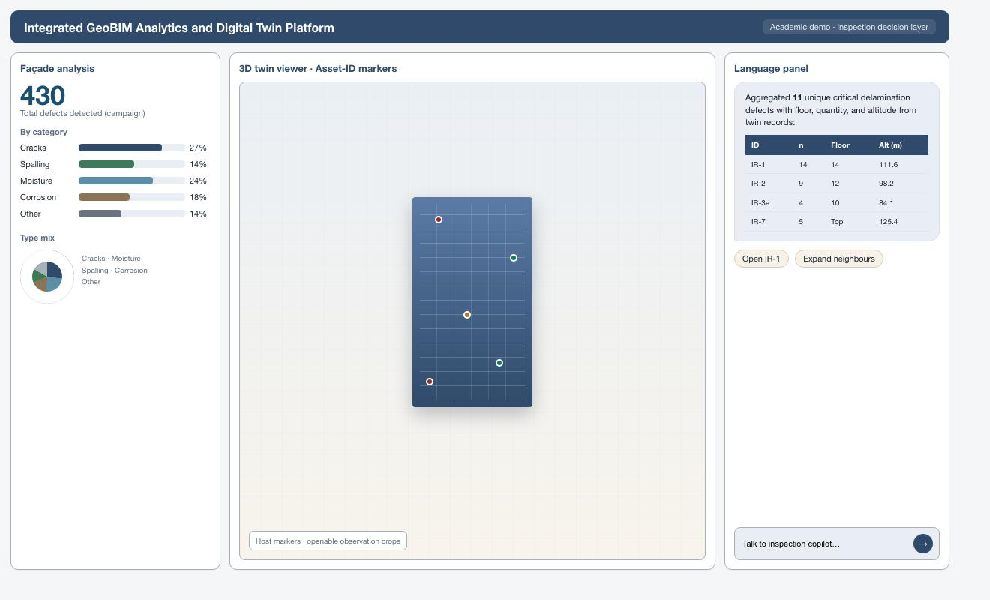
\includegraphics[width=0.82\textwidth]{platform_demo.pdf}
\caption{自然语言查询与报告起草的孪生界面示例。展示为界面模式，而非产品宣称。}
\label{fig:ch8-platform}
\end{figure}

\begin{figure}[t]
\centering

\includegraphics[width=0.88\textwidth]{multi_platform_field_interfaces.pdf}
\caption{保持现场与孪生之间 Asset-ID 一致的现场界面。}
\label{fig:ch8-field-ui}
\end{figure}

\subsection{现场身份卫生}
当现场标签与孪生 ID 分叉时，语言质量会崩塌。因此注册审计（图\ref{fig:ch8-asset-id}）属于决策层，而不是事后 IT 补丁——这与 GeoBIM 时代的孪生实践一致~\cite{zhang2025}。

\begin{figure}[t]
\centering

\includegraphics[width=0.85\textwidth]{field_asset_id_stages.pdf}
\caption{现场采集与检索之间的分阶段 Asset-ID 核验。}
\label{fig:ch8-asset-id}
\end{figure}

\subsection{专栏~8.1：端到端自然语言演示}
\begin{tcolorbox}[title={专栏 8.1 —— 从问题到可审计草稿}, breakable, colback=black!3, colframe=black!55]
\textbf{问题（设施经理）.}
「东立面 A-07 板块似乎有渗水向上爬升。上方两层哪些资产应优先安排吊篮，并能起草一份我可审计的维修简报吗？」

\textbf{步骤1——意图.}
分类器标记为\emph{传播 + 规划}。种子资产 $=\{$A-07$\}$；请求跳数 $k=2$；关注模态 $=$ RGB 与 IR。

\textbf{步骤2——检索.}
\texttt{get\_passport(A-07)} 返回观测 $o_1$（RGB 裂缝，置信度 0.91）与 $o_2$（IR 异常，置信度 0.84），均已配准到 A-07。手册条款留在独立专家库，此时尚未加载。

\textbf{步骤3——扩展.}
\texttt{expand\_neighbours(A-07, $k$=2)} 得到竖向链 A-07 $\rightarrow$ A-18 $\rightarrow$ A-29 以及侧向邻域 A-08、A-06。带潮湿相关症状的护照装入上下文；无关资产丢弃。

\textbf{步骤4——冲突检查.}
在 A-18 上，RGB 显示表面污渍而 IR 偏弱。拓扑助手标记 \texttt{modality\_conflict=true}，而不是断言内部渗漏。

\textbf{步骤5——生成（cite-or-abstain）.}
报告文书填充表\ref{tab:ch8-schema}：
\begin{itemize}[leftmargin=*,nosep]
\item \texttt{asset\_ids} = \{A-07, A-18, A-29\}（均 $\subseteq$ 检索集）；
\item \texttt{propagation} = 带证据 ID $o_1,o_2,\ldots$ 的竖向路径；
\item \texttt{priority} = A-29 高（叠加症状），A-18 中（冲突标记）；
\item \texttt{human\_check} = A-18 必需。
\end{itemize}
不允许出现检索集之外的 Asset-ID。若 A-29 没有任何观测，文书应对该 ID 拒答，而不是虚构严重度。

\textbf{步骤6——行动提议（门控）.}
行动提议者为第2--3章发出复访多边形提示，并给出吊篮顺序草稿。在人工批准前，\textbf{不}调度无人机，也\textbf{不}写孪生~\cite{luo2025llmdtrobot}。

\textbf{交付物.}
一份可审计简报：每条主张都能在孪生界面打开证据 URI；冲突可见；不可逆动作停在闸门之后。
\end{tcolorbox}

\paragraph{过渡.}
最后讨论决策支持评价——标准在前，案例数字在后。

%%%%%%%%%%%%%%%%%%%%%%%%%%%%%%%%%%%%%%%%%%%%%%%%%%%%%%%%%%%%%%%%%%%%%%
\section{决策支持与预测性维护}
\label{sec:ch8-dss}

\subsection{书中应评价什么}
专著读者需要可迁移的标准——而不是一张胜负柱状图：

\begin{figure}[t]
\centering
\begin{tikzpicture}[
  c/.style={draw, rounded corners=2pt, align=center, minimum height=1.2cm, minimum width=2.35cm, font=\scriptsize, fill=black!4}
]
\node[c] (c1) {接地\\被引ID$\in$集合};
\node[c, right=0.3cm of c1] (c2) {拓扑\\敏感性};
\node[c, right=0.3cm of c2] (c3) {语料\\忠实度};
\node[c, right=0.3cm of c3] (c4) {运维\\可用性};
\node[c, right=0.3cm of c4] (c5) {智能体\\安全};
\end{tikzpicture}
\caption{孪生接地语言系统的评价标准清单。优先用这些透镜，而不是单篇论文的柱状图。}
\label{fig:ch8-eval-criteria}
\end{figure}

\begin{itemize}[leftmargin=*]
\item \textbf{接地：}被引 ID 是否在证据集中？~\cite{ji2023,shuster2021}
\item \textbf{拓扑敏感性：}纳入邻域后，传播类问题是否改善？
\item \textbf{语料忠实度：}对规范/手册，RAG 是否优于纯参数回忆？~\cite{lee2024ragsafety,joffe2025buildingcodes}
\item \textbf{运维可用性：}输出能否驱动排程（吊篮、复访）？
\item \textbf{智能体安全（新兴）：}在批准与 geofence 约束下的工具成功率~\cite{luo2025llmdtrobot,rawat2025llmmas}。
\end{itemize}

\subsection{案例快照（示意）}
已发表的社区评测已表明结构化检索有帮助：缺陷管理混合 RAG~\cite{jeon2025hybridrag}、安全/规范 RAG~\cite{lee2024ragsafety,joffe2025buildingcodes}、设施文档 RAG~\cite{krutli2025fmrags}。另有课题组面向物流仓立面的进行中实验（尚未同行评议发表，故不列入参考文献）在使用资产护照与邻域扩展时呈现示意性的多跳收益——适合用来教学「结构为何重要」，而非当作普适常数。下列图因此标注为\emph{示意性案例草图}，而不是本章的科学主脊。

\begin{figure}[t]
\centering

\includegraphics[width=0.78\textwidth]{deterministic_ablation_exact_hit.pdf}
\caption{示意性案例消融草图（可选阅读）：去掉资产结构或邻域扩展时，多跳题受损最大。}
\label{fig:ch8-ablation}
\end{figure}

\begin{figure}[t]
\centering

\includegraphics[width=0.78\textwidth]{deterministic_external_exact_hit.pdf}
\caption{在共享「仅观测」协议下，案例与常见 RAG 基线的示意对照。}
\label{fig:ch8-external}
\end{figure}

\begin{figure}[t]
\centering

\includegraphics[width=0.75\textwidth]{hallucination_rate.pdf}
\caption{案例视角：无支持主张 vs 接地配置。}
\label{fig:ch8-halluc}
\end{figure}

\begin{figure}[t]
\centering

\includegraphics[width=0.75\textwidth]{deterministic_ksweep_coverage.pdf}
\caption{示意性 $k$ 跳扫描：传播类问题覆盖率随邻域半径变化。用来教学 $k$ 的运维含义，而非当作普适最优。}
\label{fig:ch8-ksweep}
\end{figure}

\subsection{预测性与跨域使用}
优先级评分与运维规划把诊断转成排程。改造排序、施工监测等迁移想法出现在 DT/智能体项目中~\cite{rawat2025llmmas,luo2025llmdtrobot,lee2025multiagentvbm}，应作为\textbf{schema 复用}来教，而不是当作有保证的预测。真正的劣化预测仍需要超越单次巡检时相的时序模型。

\begin{figure}[t]
\centering

\includegraphics[width=0.82\textwidth]{framework_generalizability_concept.pdf}
\caption{孪生—语言模式在运维任务间迁移的概念示意。}
\label{fig:ch8-transfer}
\end{figure}

\subsection{开放问题}
拓扑完整度与 Asset-ID 卫生仍是主误差源。面向巡检的标准智能体基准（安全工具轨迹）仍然缺失。更强的 VLM–孪生实体接地、完全 VLM 原生的孪生、更丰富的长期智能体记忆，以及蜂群持续更新，属于第9章的\textbf{前沿展望}，并与多机规划章节衔接。建筑 LLM 的隐私与治理问题~\cite{saka2024gptconstruction,ma2026tenquestions}在投资组合尺度上仍然开放。

\paragraph{本章要点.}
\begin{enumerate}[leftmargin=*]
\item 第8章是全书决策层：消费第4--7章产物，用接地语言作答，而不是只看几何。
\item LLM/VLM 基础（Transformer、指令跟随、多模态接口）解释能力；幻觉与错误编号解释为何必须接地~\cite{vaswani2017attention,brown2020,ji2023}。
\item 记忆必须分层：权重 $\neq$ 上下文窗口 $\neq$ RAG 索引 $\neq$ 孪生库~\cite{lewis2020,krutli2025fmrags,pan2024b}。
\item 观测记录、资产护照与 $k$ 跳拓扑让检索有可靠对象；cite-or-abstain 让生成保持诚实。
\item RAG、工具/智能体与结构化资产知识彼此互补；AEC 已在 BIM、规范、FM 与安全中使用它们——立面孪生额外要求拓扑与 Asset-ID 纪律~\cite{lewis2020,zheng2023bimassistant,lee2024ragsafety,luo2025llmdtrobot,rawat2025llmmas}。
\item 报告、现场身份卫生与批准闸门，对决策支持而言与模型选择同等重要。
\end{enumerate}


% ----- 第9章：仅列章节名 -----
\StubChapter{结论与展望}

\bibliographystyle{plainnat}
\bibliography{references}

\end{document}
